\section{Unit Testing}
\begin{mdframed}
    \textbf{Unit Testing:} Il testing di unità è il collaudo di singole unità software. Per unità si intende il minimo componente diun programma dotato di funzionamento autonomo (può essere una classe o una funzione a seconda del paradigma di programmazione).
\end{mdframed}
Può essere sia manuale che automatico. Specialmente nel caso dello Unit Testing automatico, lo sviluppo dei test case è considerato parte integrante dell'attività di sviluppo.
  
\subsection{A TRIP}

\subsubsection{Automatic}
I test di unità devono essere eseguiti automaticamente. In ogni progetto deve essere disponibile un “automazione a comando” che permetta a tutti di invocare e far eseguire tutti o una parte dei test di unità in modo semplice.
Durante la fase di sviluppo del progetto è importante che i test possano essere eseguiti:
\begin{itemize}
    \item \textbf{In modo rapido:} i test devono essere semplici e la loro esecuzione deve richiedere pochi secondi.
    \item \textbf{Senza richiedere l'interazione umana:} il test non deve richiedere l'intervento umano, ad esempio per passare deiparametri.
    \item \textbf{In modo autonomo:} gli sviluppatori devono essere avvisati solo quando viene riscontrato un errore.
\end{itemize}

\subsubsection{Thorough}
Dei buoni test di unità devono essere esaustivi e accurati, devono verificare il comportamento di qualsiasi parte del progetto che potrebbe creare degli errori.
Esistono degli strumenti che permettono di misurare se ogni parte del progetto è stata
eseguita durante la fase di test, e possono calcolare:
\begin{itemize}
    \item Percentuale di righe di codice
    \item Percentuale di possibili diramazioni
    \item Numero di eccezioni
\end{itemize}

\subsubsection{Repeatable}
I test di unità devono produrre sempre lo stesso risultato.
Per essere ripetibili, i test di unità devono avere le seguenti caratteristiche:
\begin{itemize}
    \item \textbf{Indipendenti dall'ordine di esecuzione:} l'ordine di esecuzione dei test di unità non deve influenzare il risultato. Per questo è necessario che i test siano indipendenti
    \item \textbf{Indipendenti dall'ambiente di esecuzione:} l'esecuzione dei test non deve dipendere da risorse esterne al progetto. Se alcune unità usano risorse esterne, è consigliato usare dei Mock Object per simulare il comportamento di queste componenti.
\end{itemize}

\subsubsection{Independent}
I test di unità devono essere indipendenti dall'ambiente di esecuzione, da elementi esterni al progetto e dall'ordine diesecuzione. Quando si scrive un test è consigliato verificare il comportamento di un singolo aspetto del progetto peridentificare univocamente l'errore. Se il test è indipendente, il suo comportamento sarà ripetibile nel tempo perchè non dipenderà dalle altre unità del progetto.

\subsubsection{Professional}
Devo essere scritti e manutenuti con lo stesso rigore con cui si scrive il codice di produzione. Il numero di righe di codice di test dovrebbe essere maggiore o uguale delle linee di codice in produzione.

\subsection{Framework}
Per creare i test di unità si sfruttano dei framework, con le seguenti caratteristiche:
\begin{itemize}
    \item Configurazione l'ambiente di esecuzione del test.
    \item Selezione di un test o un insieme di test da eseguire.
    \item Analizzazione di valori aspettati, prodotti dalle unità.
    \item Standard per esprimere se il test è stato superato, se è fallito o se sono stati prodotti degli errori.
\end{itemize}

\subsection{Right BICEP}

\subsubsection{Rigth}
Dobbiamo porci la domanda "Are the results right?". In caso di ambiguità nei requisiti, i test di unità sono un buon punto di partenza per documentare il codice, ossia per documentare in che modo losviluppatore ha interpretato i requisiti e descrivere il comportamento delle unità realizzate.

\subsubsection{Boundary Conditions}
Solitamente gli errori accadono nelle condizioni limite, dove il programmatore non ha prestato attenzioni ai dettagli.
Identificare le condizioni limiti è una delle parti più importanti nella creazione dei test di unità.
I risultati devono essere \textbf{CORRECT}
\begin{itemize}
    \item \textbf{C}onformance: i valori sono conformi al formato atteso?
    \item \textbf{O}rdering: i valori seguono o no un ordine?
    \item \textbf{R}ange: i valori sono dentro un minimo o massimo appropriato?
    \item \textbf{R}eference: i valori possono provenire da dati esterni non sotto il controllo del codice?
    \item \textbf{E}xistence: i valori esistono? non nulli, non zero, appartenenti ad un determinato insieme?
    \item \textbf{C}ardinality: i valori sono nella quantità desiderata?
    \item \textbf{T}ime: i valori rispettano un ordine temporale?
\end{itemize}

\subsubsection{Check Inverse Relationship}
Alcune unità possono essere controllate tramite l'applicazione della loro funzionalità inversa.
Per esempio la radice quadrata: per testare una radice quadrata, elevo al quadrato l'output dell'unità e lo confronto col valore di input.

\subsubsection{Cross-check Using Other Means}
Usare un oracolo per verificare se la nuova unità ha lo stesso comportamento.
Uso il vecchio sistema per verificareche il nuovo abbiamo lo stesso comportamento.

\subsubsection{Force Error Condition}
Nel mondo reale gli errori esistono e devono essere gestiti, per tanto è buona norma ricreare le condizioni di errore everificare che il progetto funzioni come previste in queste condizioni.

\subsubsection{Performace Characteristic}
Devono essere veloci perchè vengono eseguiti molto spesso.

\subsection{TDD}
Modello di sviluppo software che prevede che la stesura dei test automatici avvenga prima di quella del software, che deve essere sottoposto a test, e che lo sviluppo del software applicativo sia orientato esclusivamente all'obbiettivo di passare i test automatici precedentemente disposti.
\begin{enumerate}
    \item \textcolor{red}{(Re)Write a Test} [rossa]: scrivi il test per la nuova funzione. Se ha successo riscrivi il test, se fallisce scrivi il codice
    \item \textcolor{green}{Write Production Code} [verde]: sviluppa la quantita minima di codice per passare il test. Se fallisce, riscrivi il codice. Se riesce, pulisci il codice
    \item \textcolor{gray}{Clean Up Code} [grigia]: migliora la qualità de codice
\end{enumerate}
\begin{center}
    \begin{tabular}{c}
        \\ 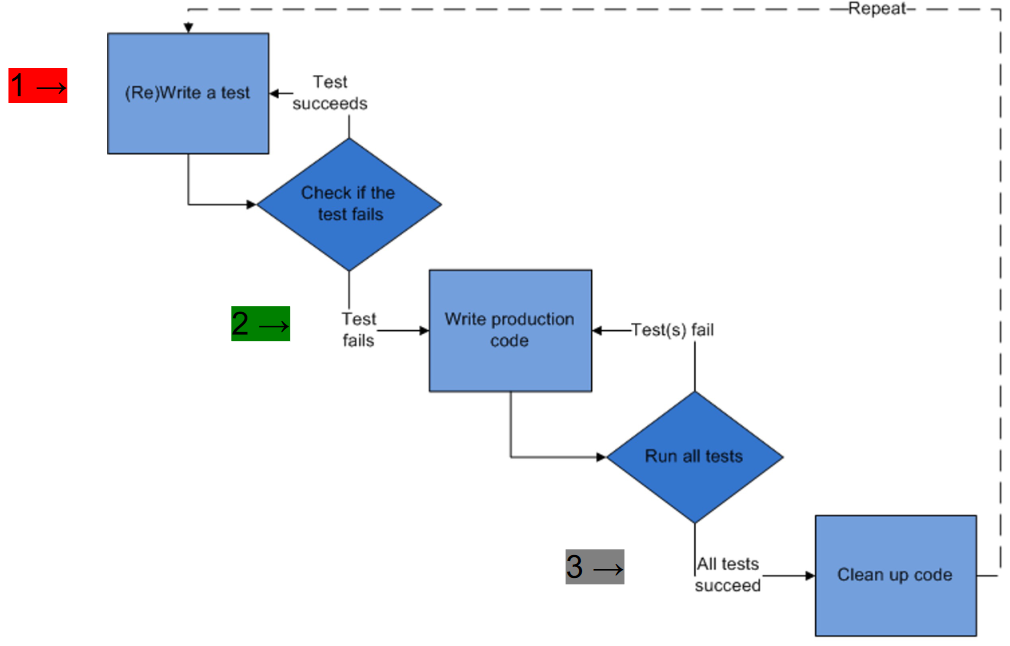
\includegraphics[width=0.9\textwidth]{images/UnitTesting1.png} \\ \\
    \end{tabular}
\end{center}

\newpage